\subsection{Présentation de \textsc{Disa}}

\subsubsection{Historique}

En 1902, une firme allemande fabriquant des décalcomanies industrielles crée une succursale à
Paris : <<~Auto décors~>>.

L’année 1914 mettant un terme aux relations avec l’Allemagne, M. \textsc{Lacarrière}, alors directeur, achète un petit atelier rue Boileau, à Limoges.
Huit ans plus tard, les bénéfices engendrés lui permettent de racheter le fonds de commerce de la société et il fonde la manufacture de \textsc{Décalcomanies Industrielle SA}.

De 1922 à 1965, l’entreprise prospère jusqu’à devenir la première fabrique de décalcomanies en France.
L’atelier rue Boileau, pourtant aménagé sur 3 étages, ne suffit plus.
La société entreprend un déménagement dans la zone industrielle de Magré-Romanet, à Limoges.
Au cours des trente années qui suivent, aucune évolution majeure n’est à noter.
Divers travaux étendent la superficie du bâtiment à 8600 m$^2$ et l’entreprise continue de se développer.
L’activité est tournée à 70 \% vers l’industrie et 30 \% vers le milieu publicitaire.

En 1995, à la suite d’un dépôt de bilan, Christophe \textsc{Renard}, le PDG associé à Patrick \textsc{Turpin}, ont repris cette entreprise de marquage industriel en difficulté, afin de disposer de leur propre solution de marquage dans le domaine de la signalétique et de l'automobile.
L'ensemble du personnel, soit 130 salariés, a été repris, de même que les locaux et les machines, ainsi l'activité a pu se poursuivre dans le même secteur d'activité.

En 2006, Jean François \textsc{Archer}, directeur général de \textsc{Disa}, envisage de déplacer une partie de l’usine dans de nouveaux locaux.
Ce processus est accéléré en 2007 par l’arrivée d’une nouvelle activité au sein de \textsc{Disa} exigeant une surface au sol importante, la PLV~:~Publicité sur Lieu de Ventes.

En 2008, le déménagement d’une partie des outils de production et du personnel se fait dans de nouveaux locaux, à 200 mètres de \textsc{Disa}, c'est la naissance de \textsc{Disa Technology}, qui est abrégé en \textsc{DisaTech}.
Cette décision est prise dans le but de séparer les deux secteurs de clientèle principaux.
Cela permettra d’accélérer la réactivité et d'accroître la productivité.

\textsc{DisaTech} est orientée vers le secteur industriel, tandis que le milieu publicitaire continue
d’être géré par \textsc{Disa}.

En 2011, \textsc{Serica Communication} basée à Nancy rejoint le groupe \textsc{Disa} et complète son offre en sérigraphie grand format grâce à son parc de machines uniques.
Malheureusement, la situation financière de \textsc{Serica} n'est pas idéale et la société est liquidée en 2018.

En 2018, la société \textsc{DisaTech} est rachetée par le groupe international \textsc{AkzoNobel}.
Cela a pour effet la mutation de nombreux employés de \textsc{Disa} vers \textsc{DisaTech}, dont mon tuteur en entreprise, M. Florent \textsc{Palier}.
M. Jean François \textsc{Archer} n'est désormais plus le directeur général de \textsc{Disa}, il est passé directeur à \textsc{DisaTech}.
Au sein de \textsc{Disa}, M$^{me}$ Sylvie \textsc{Jarraud} est devenue responsable administrative et comptable, M. Patrick \textsc{Mery} est maintenant directeur de la production et M. Bertrand \textsc{Cotteret} est directeur commercial.

\newpage
\subsubsection{Le métier d’imprimerie}

La société \textsc{Disa} est une imprimerie de labeur, elle traite des travaux d'impression publicitaire.
Certains clients demandent la création de modèles en 3 dimensions, pour de l'exposition de produits notamment, \textsc{Disa} est donc en mesure de proposer des produits en volume ou non.

\FloatBarrier
\begin{figure}[h!]
    \begin{center}
        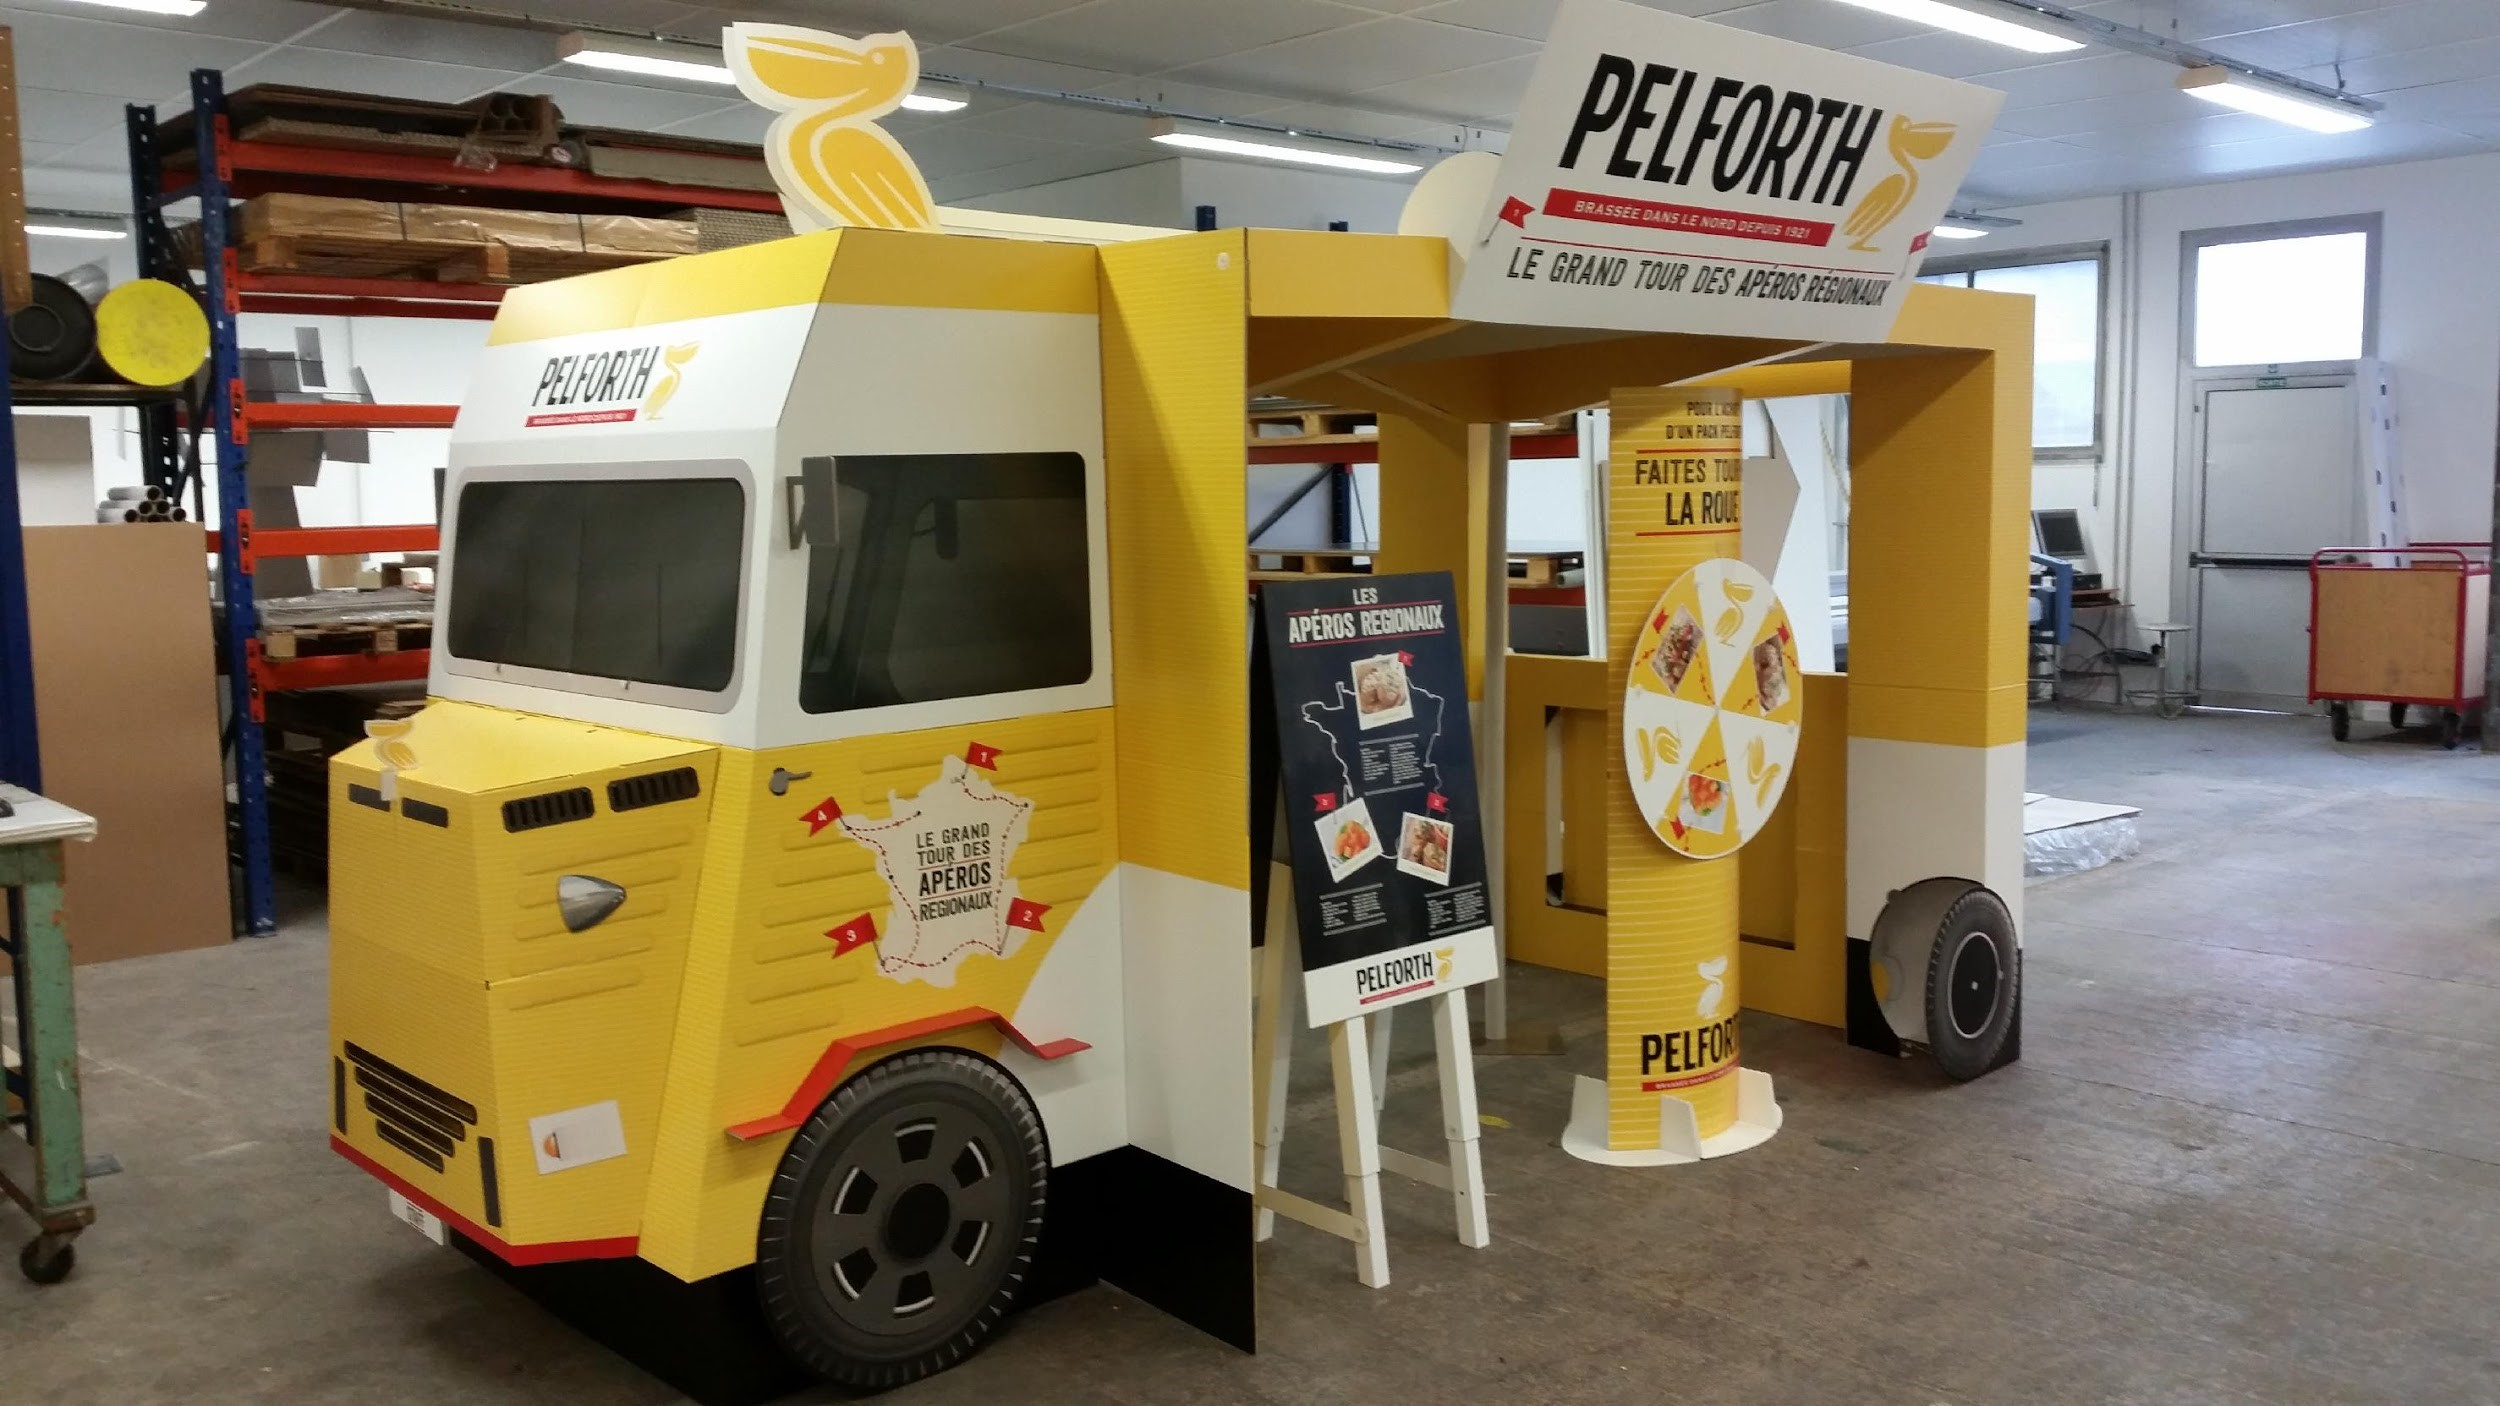
\includegraphics[width = 0.5\textwidth]{camion}
    \end{center}
    \caption{Camion en carton, PLV 3D}
    \label{figure:plv3d}
\end{figure}
\FloatBarrier

Ses produits sont basés sur trois techniques d'impression présentant toutes des avantages et inconvénients différents~:~
\\
\begin{itemize}
    \item[\tiny$\bullet$] \textbf{La sérigraphie~:}~Cette méthode est basée sur des pochoirs qui sont placés entre l'encre et le support d'impression.
    Cette technique permet l'utilisation de n'importe quel type de support.
    Les écrans utilisés en tant que pochoir offrent une taille d'impression conséquente.
    Cette méthode est assez lente, mais offre une qualité d'impression difficilement atteignable avec les autres méthodes.
    
    \item[\tiny$\bullet$] \textbf{L'offset~:}~Cette méthode nécessite la création d'une plaque en aluminium sur laquelle est gravé le motif voulu.
    Une fois la plaque créée, elle est installée sur un cylindre dans la machine.
    Celle-ci peut ensuite imprimer des feuilles à la chaîne à une vitesse extrêmement rapide.
    Cette méthode est donc idéale lorsqu'il faut imprimer un nombre important d'exemplaires d'un même motif.
    Les supports d'impression utilisés sont généralement de l'adhésif ou du PVC.
    
    \item[\tiny$\bullet$] \textbf{Le numérique~:}~Cette méthode utilise le même principe qu'une imprimante de bureau à jet d'encre.
    Ce procédé est très précis, mais assez lent (150 fois plus lent que l'offset).
    En revanche, contrairement aux deux autres méthodes celle-ci ne nécessite pas de travail en amont et quasiment aucune intervention de la part des ouvriers sur la machine.
\end{itemize}
~\\

Selon le cahier des charges des clients, la méthode d'impression la plus efficace est utilisée.
